% Template article for preprint document class `elsart'
% with harvard style bibliographic references
% SP 2006/04/26

\documentclass[preprint,twocolumn,authoryear,5p]{elsarticle}

\newcommand{\fv}{\mbox{\boldmath $f$}}
\newcommand{\Iv}{\mbox{\boldmath $I$}}
\newcommand{\xv}{\mbox{\boldmath $x$}}
\newcommand{\velocity}{\mbox{\boldmath $v$}}
\newcommand{\velocityinv}{\mbox{\boldmath $v$}^{-1}}
\newcommand{\Velocityinv}{\mbox{\boldmath $V$}^{-1}}
\newcommand{\Velocity}{\mbox{\boldmath $V$}}
\newcommand{\welocity}{\mbox{\boldmath $w$}}
\newcommand{\spatialimagegradient}{\mbox{\boldmath $I$}\mbox{$_{x}$}}
\newcommand{\perpspatialimagegradient}{\mbox{\boldmath $I$}\mbox{$^{\perp}_{x}$}}
\newcommand{\temporalimagederivative}{\mbox{$I_t$}}
\newcommand{\finitestrain}{\mbox{\boldmath $\varepsilon^{\ast}$}}
\newcommand{\smallstrain}{\mbox{\boldmath $\varepsilon$}}
\newcommand{\dispgradient}{{\bf \nabla \displace}}
\newcommand{\displace}{{\bf u}} 
\newcommand{\Id}{\text{\bf Id}}
\newcommand{\ode}{{\em O.D.E.}}
\newcommand{\odes}{{\em O.D.E.}s}
\newcommand{\G}{\mathcal{G}}
\newcommand{\J}{\mathcal{J}}
\newcommand{\phiinv}{\phi^{-1}}
\newcommand{\psiinv}{\psi^{-1}}
\newcommand{\dM}{DM}
\newcommand{\DM}{Diffeomorphometry}
\newcommand{\diff}{diffeomorphism}
\newcommand{\Diff}{Diffeomorphism}
\newcommand{\orbit}{\mathcal{O}}
\newcommand{\avg}{\mathcal{A}}
\newcommand{\avgn}{\mathcal{A}_n}
\newcommand{\avgna}{\mathcal{A}^a_{n}}
\newcommand{\nset}{\{ J_i \}_n}
\newcommand{\bari}{\bar{I}}
\newcommand{\bart}{\bar{t}}
\newcommand{\jac}{\mathcal{J}}
\newcommand{\pert}{\mbox{\boldmath $w$}}
\newcommand{\barpert}{\bar{\mbox{\boldmath $w$}}}
\newcommand{\half}{0.5}

\newcommand{\X}{{\bf X}}
\newcommand{\x}{{\bf x}}
\newcommand{\Z}{{\bf Z}}
\newcommand{\z}{{\bf z}}
\newcommand{\p}{{\bf p}}
\newcommand{\Y}{{\bf Y}}
\newcommand{\y}{{\bf y}}
\newcommand{\ytild}{\tilde{{\bf y}}}
\newcommand{\q}{{\bf q}}
\newcommand{\surf}{\mathcal{S}}
\newcommand{\phij}{\phi_{ij}}
\newcommand{\aphij}{\bar{\phi}_{j}}
\newcommand{\apsij}{\bar{\psi}_{j}}
\newcommand{\aphi}{\bar{\phi}}
\newcommand{\aphiinv}{\bar{\phi}^{-1}}

\newcommand{\domain}{\Omega}
\newcommand{\meanshape}{\bf \bar{x}}
\newcommand{\g}{\mbox{\boldmath $g$}}
\newcommand{\h}{\mbox{\boldmath $h$}}
\newcommand{\yv}{\mbox{\boldmath $y$}}

\newcommand{\group}{Diff}


\newcommand{\evol}{{E_{\text{Vol}}}}
\newcommand{\epair}{{E_{\text{Pair}}}}
\newcommand{\esec}{{E_{S}}}
\newcommand{\inv}{^{-1}}
\newcommand{\vinit}{ \velocity^0_{ij}(\x,\tau=0) }
\newcommand{\avinit}{ \bar{\velocity}^0_{j}(\x,t) }
\newcommand{\avinitz}{ \bar{\velocity}^0_{j}(\x,t_a) }
\newcommand{\gz}{\nabla_{\z}}

\newcommand{\Section}[1]{\vspace{-8pt}\section{\hskip-1em.~~#1}\vspace{-3pt}}
\newcommand{\SubSection}[1]{\vspace{-3pt}\subsection{\hskip -1em.~~#1}\vspace{-3pt}}

\newcommand{\BASE}{.}%/Users/stnava/Work/}
\newcommand{\TEXDIR}{.}%{\BASE Words/Writing/}
\newcommand{\ROOT}{.}%{\BASE Words/}
\newcommand{\FIGDIR}{.}%{\BASE Words/Writing/MEDIAITK/wbir/}
\newcommand{\FIGDIRAIBS}{.}%{\BASE Words/Writing/IPMI2003/jpegs/}
\newcommand{\FIGDIRP}{proposal/}%{\BASE Words/Writing/proposal/}
\newcommand{\FIGDIRPJ}{proposal/jpegs/}%{\BASE Words/Writing/proposal/jpegs/}
\newcommand{\FIGDIRADAD}{.}%{\BASE Words/Writing/ADAD/}
\newcommand{\FIGS}{.}%{\BASE Words/Writing/neuroimageipam-final/FIGS/}


% Use the option doublespacing or reviewcopy to obtain double line spacing
 %\documentclass[doublespacing]{elsart}

% the natbib package allows both number and author-year (Harvard)
% style referencing;
\usepackage{natbib}

% if you use PostScript figures in your article
% use the graphics package for simple commands
% \usepackage{graphics}
% or use the graphicx package for more complicated commands
 \usepackage{graphicx}
% or use the epsfig package if you prefer to use the old commands
% \usepackage{epsfig}

% The amssymb package provides various useful mathematical symbols
\usepackage{amssymb,amsmath}
\usepackage{color}
\usepackage{algorithm}
\usepackage{algorithmic}
\usepackage{rotating}
\usepackage{multirow,booktabs,ctable,array}
\usepackage{listing}						
\usepackage{listings}					

\graphicspath{{/Users/nick/Documents/Academic/Gee/SubmittedPapers/JournalPapers/MedIA2009_BrianANTS/Figures/}
%{/Users/nick/Documents/Academic/Gee/SubmittedPapers/Conferences/ISBI2007/Images/}
%                          {/Users/nick/Documents/Academic/Gee/Projects/Helium-3/GrantSubmissions/R21/resplan/Images/}
%                          {/Users/nick/Documents/Academic/Gee/SubmittedPapers/JournalPapers/MRM2008/Figures/}
%                          {/Users/nick/Documents/Academic/Gee/SubmittedPapers/Conferences/ISBI2008/Figures/}
                          }

% The lineno packages adds line numbers. Start line numbering with
% \begin{linenumbers}, end it with \end{linenumbers}. Or switch it on
% for the whole article with \linenumbers.
 \usepackage{lineno}

%\linenumbers
\begin{document}


%Setup listing environment
\definecolor{listcomment}{rgb}{0.0,0.5,0.0}
\definecolor{listkeyword}{rgb}{0.0,0.0,0.5}
\definecolor{listbackground}{gray}{0.965}

\lstset{frame = tb,
        framerule = 0.25pt,
        float,
        fontadjust,
        backgroundcolor={\color{listbackground}},
        basicstyle = {\ttfamily\scriptsize},
        keywordstyle = {\ttfamily\color{listkeyword}\textbf},
        identifierstyle = {\ttfamily},
        commentstyle = {\ttfamily\color{listcomment}\textit},
        stringstyle = {\ttfamily},
        showstringspaces = false,
        showtabs = false,
        numbers = none,
        tabsize = 2,
        language=[ISO]C++,
        floatplacement=!h
        }	


\begin{frontmatter}

% Title, authors and addresses

% use the thanksref command within \title, \author or \address for footnotes;
% use the corauthref command within \author for corresponding author footnotes;
% use the ead command for the email address,
% and the form \ead[url] for the home page:
% \title{}
% \thanks[label1]{}
% \author{Name\corauthref{cor1}\thanksref{label2}}
% \ead{tustison@grasp.cis.upenn.edu}
% \ead[url]{home page}
% \thanks[label2]{}
% \corauth[cor1]{}
% \address{Address\thanksref{label3}}
% \thanks[label3]{}

\title{ANTS:  Advanced Open-Source Tools for Normalization And Neuroanatomy}
\author[label1]{PICSL}

% use optional labels to link authors explicitly to addresses:
% \author[label1,label2]{}
\address[label1]{Penn Image Computing and Science Laboratory, University of Pennsylvania, Philadelphia, PA, USA}
%\address[label2]{Department of Mathematics, University of Pennsylvania, Philadelphia, PA, USA}


\begin{abstract}
Computational anatomy (CA) seeks to quantify natural variation in
biological shape and function with roots that reach back to the
seminal works of Charles Darwin and D'arcy Thompson.  CA is currently
applied to study health, disease and epidemiology and uses deformable
mappings between images as a basic technique.  However, there is a
lack of standards and reproducibility in the field that is due, in
part, to the use of proprietary software and private data.  To
facilitate reproducibility in CA measurements and advancement of
imaging sciences, NIH has recently committed significant support to
open-source data and software resources.  Here, we report a recent
product of this commitment: Advanced Normalization Tools (ANTS), an
ITK-based toolkit for CA and related areas.  The ANTS open-source
library consists of a well-evaluated suite of state-of-the-art
normalization and template-building tools for quantitative
morphometric analysis.  We highlight the prominent features of ANTS
and demonstrate its utility by performing a detailed analysis on
openly-available anatomically labeled brain data from the non-rigid
image registration evaluation project (NIREP).  The results from this
analysis evidences the high level of accuracy achievable with ANTS
using intensity-based registration alone.  In addition, we show the
significant performance gains may be achieved by coupling
intensity-based image metrics and point-set-based metrics from
specific, sensibly selected cortical structures.
%Computational anatomy is the quantitative study of biological shape and its natural variations which traces its roots to the seminal works of Charles Darwin and D'arcy Thompson.  Integral to this research field is the calculation of deformable mappings between images that serve as invaluable measurement tools.  Technological evolution has spawned much innovation in the computational development of such deformable mapping algorithms.  However, not only is algorithmic development essential for increasing scientific knowledge but the availability of these technologies is equally crucial for facilitating the progress of the scientific community at large.  This is the motivation behind such projects as the Insight Toolkit (ITK) of the National Institutes of Health which serves as a repository for many popular image segmentation and registration routines.  In addition, the ITK library provides a well-structured framework for several stand-alone projects such as Elastix, ITK-SNAP, ManagedITK, the Medical Imaging Toolkit (MITK), WrapITK, and many others.  Our own  contribution to the field of computational anatomy, also built on an ITK foundation, is called Advanced Normalization Tools (ANTS).  The ANTS open-source library consists of an entire suite of state-of-the-art normalization and template-building tools for quantitative morphometric analysis. After highlighting the prominent features of ANTS, we demonstrate its utility by performing a detailed analysis on anatomically labeled brain data from the non-rigid image registration evaluation project (NIREP).  The results from this analysis evidences the high level of accuracy achievable with ANTS using intensity-based registration alone.  In addition, we show the performance gains achieved by coupling intensity-based image metrics and point-set-based metrics from specific, sensibly selected cortical structures.
  
%In a recent evaluation of 14 non-linear deformation algorithms \cite{Klein2009}, the SyN algorithm of ANTS was consistently one of the top performers.

\end{abstract}

\begin{keyword}
ANTS \sep image registration \sep nueroanatomy \sep neuroimaging \sep normalization \sep  open-source \sep point-set registration
% keywords here, in the form: keyword \sep keyword
% PACS codes here, in the form: \PACS code \sep code
\end{keyword}

\end{frontmatter}

\section{Introduction}

The rapid advancement of biological and medical imaging technologies has caused a proliferation in the development of quantitative tools for computational anatomy.  The principal tools of this emerging field are meaningful deformable mappings between images whether they be driven by similarity metrics which are intensity-based,  point-set based, or both.  Several categories of mappings have been proposed in the literature.  Of particular recent interest are diffeomorphic transformations which, by definition, preserve topology.  Topology preservation is fundamental to making comparisons between objects in the natural world as such transformations permit comparisons to be made across time points in an individual's disease process or to study development patterns across a large population.

Despite the number of proposed algorithms, our limited assessment of published research mirrors the experience of many others who prefer a working paradigm of what has been referred to as {\em reproducible research}.  As described by Dr. Kovacevic ``[reproducible research] refers to the idea that, in `computational' sciences, the ultimate product is not a published paper but, rather, the entire environment used to produce the results in the paper (data, software,etc.).''  After an informal survey of 15 published papers, she found ``none had code available'' and ``in only about half the cases were the parameters [of the algorithm] specified'' (\cite{Kovacevic2006}).  Recent discussions within the computational sciences research community, particularly among advocates of ``open science,'' have also voiced similar concerns (\cite{Yoo2005,Ibanez2006}).   In this paper, we discuss our contribution to the open-source medical image analysis research community which we call ANTS (\underline{A}dvanced \underline{N}ormalization \underline{T}ool\underline{s}).  Built on an ITK framework, this software package comprises a suite of tools for image normalization and template building based on previously published research.  

 
Perhaps the most persuasive evidence motivating the use of our contributions discussed in this paper is the recent outcome of a large-scale comparative image registration algorithm assessment (\cite{Klein2009}). In the largest evaluation study to date involving 14 popular non-linear registration algorithms, our Symmetric Normalization (SyN) transformation model (\cite{Avants2008}) discussed below, was consistently one of the top two performers across all tests.  Overlap and distance measures used for assessment employed three completely independent analysis methods (permutation tests, one-way ANOVA tests, and indifference zone ranking).  Unlike some of the other algorithms used in this brain registration evaluation study, all of our methods (not just SyN) are available as open-source.  

We first provide an overview of the different components included in ANTS, such as the available transformation models and similarity metrics offered.  We follow this up with an extensive validation \ldots

\section{Theoretical Overview of ANTS}
A useful classification schema of normalization techniques is based upon the following three principal components (\cite{Brown1992,Ibanez2002}):
\begin{itemize}
  \item the {\em transformation model},
  \item the {\em similarity (or correspondence) measures},  and
  \item the {\em optimization strategy}.
\end{itemize}
In general, image normalization is the process of finding the optimal transformation, $\phi$, within a specified transformation space which maps each $\mathbf{x}$ of image $\mathcal{I}(\mathbf{x})$ to a location in image $\mathcal{J}(\mathbf{z})$ such that a specified cost function, $\mathcal{C}$, describing the similarity between $\mathcal{I}$ and $\mathcal{J}$, is minimized.   A summary of available transformation models and similarity measures are provided in Table \ref{table:chart}.  Details are given in subsequent sections.

\subsection{ANTS Transformation Models}

%\begin{figure*}
%  \centering
%    \begin{tabular}{c}
%      \includegraphics[width=170mm]{TransformationTable}
%    \end{tabular}
%  \caption{Available transformations and similarity metrics available in ANTS.  Similarity metric acronyms:  CC = cross correlation, MSQ = mean squares, MI = mutual information, JHCT = Jensen-Havrda-Charvat-Tsallis divergence, PSE = point-set expectation.  }
%  \label{fig:chart}
%\end{figure*}

\begin{table*}
  \centering
    \begin{tabular}{c c c c}
    {\bf Category} & {\bf Transformation, $\phi$} & {\bf Similarity Measures} & {\bf Brief Description} \\
    \toprule     
    \multirow{2}*{\bf Linear}
           & Rigid$^\dagger$ & MI, MSQ & Rigid registration. \\
       {} & Affine$^\dagger$ & MI, MSQ & Affine registration. \\
       \cmidrule(l){2-4}
    \multirow{2}*{\bf Elastic}
           & Deformable & CC, PR, MI, MSQ, PSE & Demons-like algorithm. \\
       {} & DMFFD & CC, PR, MI, MSQ, PSE  & FFD variant. \\
       \cmidrule(l){2-4}
    \multirow{2}*{\bf Diffeo.}
           & Exponential$^\dagger$ &  CC,PR, MI, MSQ, PSE  & $~\min~\velocity(\x)$ \\
       {} & Greedy SyN$^\dagger$ &  CC, PR, MI, MSQ, PSE  & ~~locally in time~$\min~\velocity(\x,t)$\\
       {} & Geodesic SyN$^\dagger$ &  CC, PR, MI, MSQ, PSE  &  $~\min~\velocity(\x,t)$ over all time \\
    \bottomrule
    \end{tabular}
  \caption{Transformations and a subset of the similarity metrics available in ANTS.  Similarity metric acronyms:  CC = cross correlation, PR = probabilistic matching, MSQ = mean squared difference, MI = mutual information, PSE = point-set expectation.  ANTS also provides the inverse of those transformations denoted by the `$\dagger$' symbol.  The brief descriptions of the diffeomorphic algorithms contrast the way in which the velocity field is optimized and used to parameterize $\phi$, the mapping.  All 
ANTS Diff algorithms generate $\phi(\x,t)$ over $t \in [ 0, 1]$ through gradient descent.}
  \label{table:chart}
\end{table*}    
\vspace{0in}


A variety of transformation models have been proposed in the literature with varying degrees of freedom (illustrated in Figure \ref{fig:hierarchy}).  For deformable transformations, one approach is to optimize within the space of non-topology preserving, yet physically motivated transformations---an approach pioneered by Bajcsy (\cite{Bajcsy1989}).  Elastic and related models, such as HAMMER (\cite{Shen2002}), statistical parametric mapping (SPM) (\cite{Ashburner2000}), free-form deformations (FFD) (\cite{Rueckert1999}), and
Thirion's demons (\cite{Thirion1998}) operate in the space of vector fields, which does not preserve topology.  In other words, barring ad hoc constraints to prevent otherwise, these algorithms allow the topology to change in an uncontrolled way which makes the deformable mappings difficult to interpret in functional or anatomical studies.   

These topology concerns have led to current advocation within the computational anatomy research community of diffeomorphic mappings for transformation modeling.   Optimizing directly within this space has shown remarkable success in various computational anatomy studies involving longitudinal (\cite{Avants2007b,Fox2001}), functional (\cite{Miller2005}), and population data (\cite{Avants2007b}).  We include three such diffeomorphic algorithms in the ANTS toolbox based on previously reported research.

Regardless of current research trends, however, we recognize that selection of the transformation model is ultimately application-specific, that no single choice is optimal for all scenarios (\cite{Wolpert1997}), and, therefore, the transformation model must be chosen in a principled fashion.  In fact, several non-diffeomorphic algorithms performed quite well in Klein's comparative study of nonrigid registration algorithms (\cite{Klein2009}).  For this reason, we also include elastic-related methods for a panoply of transformation model options. 

\begin{figure}
  \centering
    \begin{tabular}{c}
      % 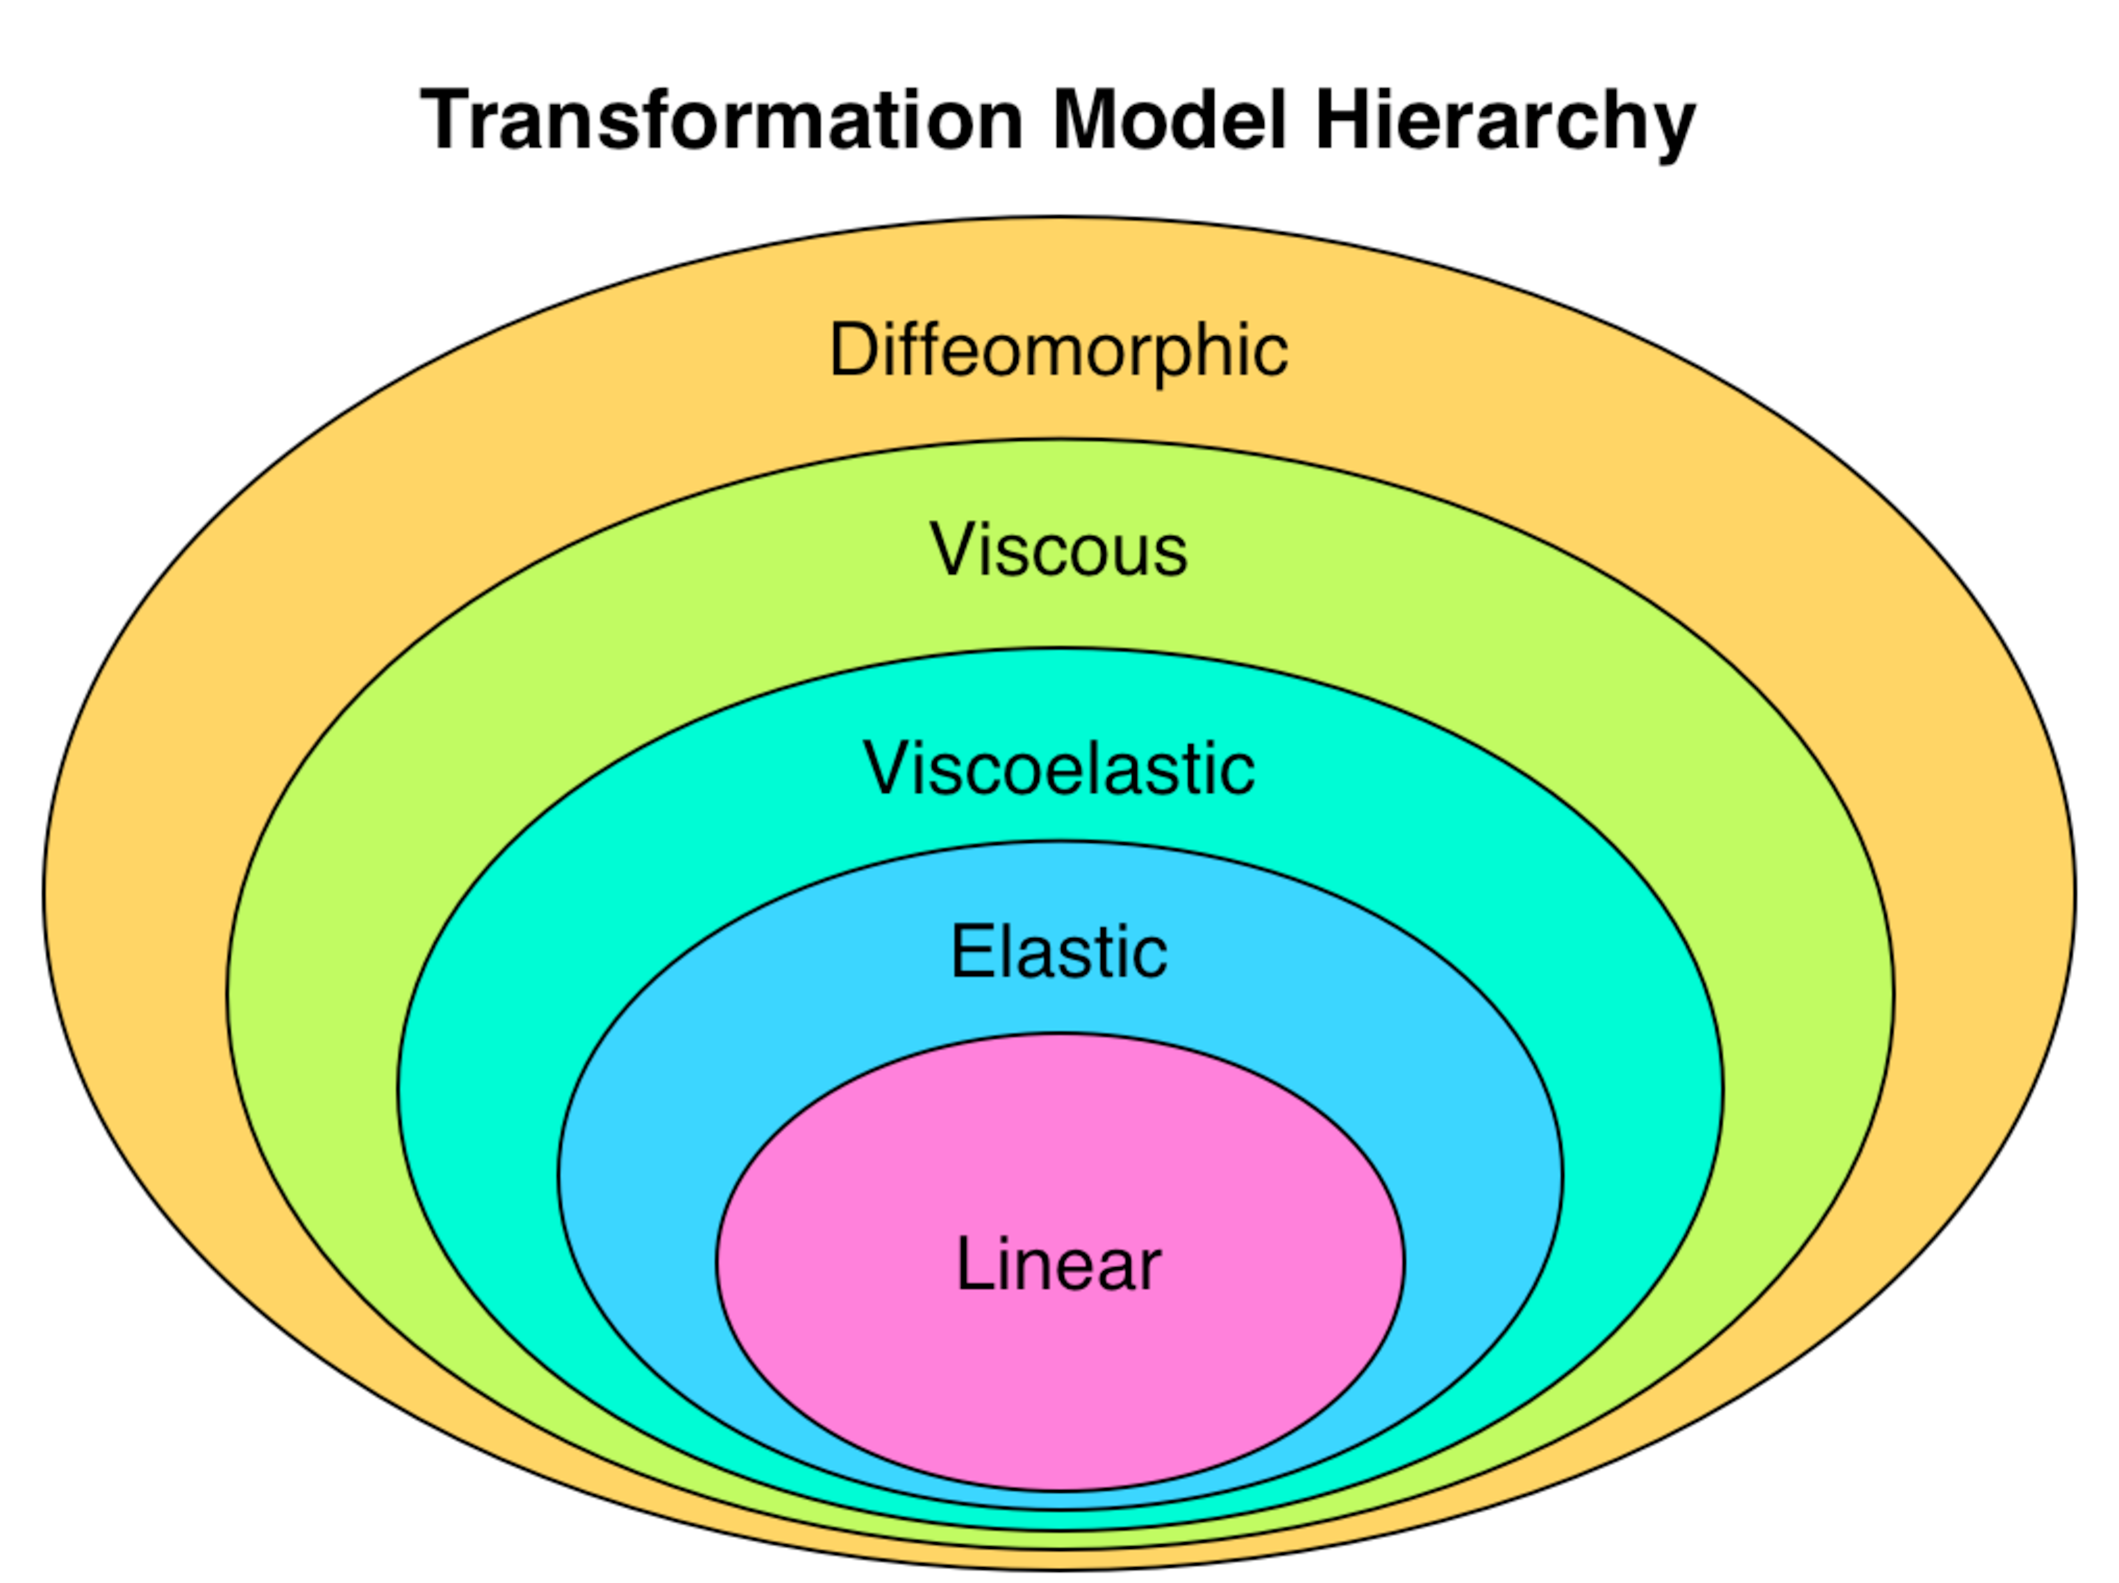
\includegraphics[width=80mm]{hierarchy}
    \end{tabular}
  \caption{Diagrammatic illustration of the transformation model hierarchy where the encompassing transformation spaces are characterized by increasing degrees of freedom.  }
  \label{fig:hierarchy}
\end{figure}



\subsubsection{Linear Transformations--Rigid and Affine:}
Image registration strategies often begin with a linear transformation
for initial global alignment which follows a deformable
transformation with increased degrees of freedom.  
Affine transformations within ANTS optimize either a
mean-squared difference metric or a mutual information (MI) image
similarity metric.  ANTS affine transformations are optimized
w.r.t. translation, rotation, scaling and shearing in succession.
This strategy allows careful control of each component of the affine
transformation.  Internally, ANTS also composes the affine
transformation with the deformation field before performing any
interpolation or downsampling.  In this way, ANTS normalization never
requires more than a single image interpolation step and is able to
always refer back to the original full-resolution image sources.

\subsubsection{Diffeomorphic Transformations}
In contrast to many transformation models which reside in the domain of vector spaces, a diffeomorphism is a differentiable mapping with a differentiable inverse (\cite{Ebin1970,Mumford1998}).  Modeling transformations with diffeomorphisms ensures certain desirable topological properties that cannot be guaranteed with other methods.  

ANTS assumes the diffeomorphism (differentiable mapping with a differentiable
inverse), $\phi$, is defined on the image domain, $\Omega$, and
maintains an affine transform at the boundary such that
$\phi(\partial \Omega) = A(\mathbf{Id})$ where $A(\mathbf{Id})$ is an
affine mapping applied to the identity transformation.  The $\phi$,
over time, parameterizes a family of diffeomorphisms,
$\phi(\mathbf{x}, t) : \Omega \times t
\rightarrow \Omega$, which can be generated by integrating a
time-dependent, regularized velocity field, $\boldsymbol{v} : \Omega \times
t \rightarrow \mathbb{R}^d$, through an ordinary differential equation
(o.d.e.).  
\begin{align} \label{eq:ode}
\frac{d \phi(\mathbf{x}, t)}{dt} = \boldsymbol{v}(\phi(\mathbf{x}, t), t), \,\,\, \phi(\mathbf{x}, 0) = \mathbf{x}.
\end{align}
The existence and uniqueness theorem for o.d.e.'s implies that integrating Equation (\ref{eq:ode}) generates a diffeomorphism.  
The deformation field provided by $\phi$ is
$\mathbf{u}(\mathbf{x})=\phi(\mathbf{x}, 1) - \mathbf{x}$.


Dupuis et al. (\cite{Dupuis1998}) motivated the usage of diffeomorphisms for CA  by showing that the variational form
\begin{align}\label{eq:D}
  D(\mathcal{I}, \mathcal{J}) =  \int_0^1 ||L\boldsymbol{v}(x,t)||^2 dt , \,\, \mathcal{I}(\phi(\mathbf{x}, 1)) = \mathcal{J}(\mathbf{z})
\end{align}
represents a true mathematical metric between anatomical instances $\mathcal{I}$ and $\mathcal{J}$ given an appropriate norm, $L$, on the velocity field, $\boldsymbol{v}$.  An optimal solution, $\boldsymbol{v}^*$, minimizes the metric $D(\mathcal{I}, \mathcal{J})$ with respect to $L$.   Dupuis (\cite{Dupuis1998}) also showed that such a solution is guaranteed to be well-posed.  Intuitively, Equation (\ref{eq:D}) provides a sense of distance between two anatomical shapes.  It also illustrates that the optimal diffeomorphic solution is analogous to finding the geodesic curve between two points in a curved space.
\footnote{
It is important to note the similarity between the definition of curve length, $\int ||\mathcal{C}'(t)||dt$, for the parametric curve $\mathcal{C}(t)$ and Equation (\ref{eq:D}).  In this sense, the solution for Equation (\ref{eq:D}) is the geodesic diffeomorphism, where $\boldsymbol{v}$ is the tangent vector of the diffeomorphism, such that the shape distance, $D$, between $\mathcal{I}$ and $\mathcal{J}$ is minimized.
}

In most real-world applications, however, a diffeomorphic path connecting the anatomical instance $\mathcal{J}$ with $\mathcal{I}$ is non-existent (due, for example, to the photometric variation or the presence/absence of a tumor in neuroanatomical images).  Therefore, the following minimizing variational form is used for optimization in diffeomorphic normalization to accommodate inexact matching  (\cite{Dupuis1998,Miller2002})
\begin{align} \label{eq:lddmm}
  \boldsymbol{v}^* = \underset{\boldsymbol{v}}{\operatorname{argmin}}  \left\{ \int_0^1  ||L\boldsymbol{v}||^2  dt + \lambda || \mathcal{I} \circ \phi(\mathbf{x},1) - \mathcal{J}  ||  \right\}.
\end{align}
The Euler-Lagrange equations characterizing the optimizing time-varying velocity field, $\boldsymbol{v}^*$, were derived in \cite{Miller2002} and later used in formulating the gradient-descent optimization scheme known as {\em large deformation diffeomorphic metric-matching} (LDDMM) (\cite{Beg2005}).   The similarity metric, or data term, for LDDMM is the {\em squared intensity difference} with weight $\lambda$.

In medical image registration, one typically encounters more complex intensity transfers 
between one anatomical instance $\mathcal{J}$ and another instance $\mathcal{I}$.  Thus, 
ANTS enables a variety of similarity terms beyond the squared difference:
\begin{align} \label{eq:diff}
  \boldsymbol{v}^* = \underset{\boldsymbol{v}}{\operatorname{argmin}}  \left\{ \int_0^1  ||L\boldsymbol{v}||^2 dt  +~\lambda~\Pi( \mathcal{I}, \phi(\mathbf{x},1) , \mathcal{J} )  \right\}.
\end{align}
Here, $\Pi$ is a similarity metric depending on the images and the
mapping and $\lambda$ controls the degree of exactness in the
matching.  If $\Pi$ is selected as cross-correlation, then one is
estimating the diffeomorphism under more robust illumination
constraints, as described in \cite{Avants2008}.  A similar equation
for elastic/FFD/DMFFD matching may be minimized in ANTS.

Exploiting the fact that the diffeomorphism, $\phi$, can be decomposed into two components 
$\phi_1$ and $\phi_2$, Avants et al. construct a {\em symmetric} alternative to Equation (\ref{eq:diff}) (\cite{Avants2007b}).  This leads to the symmetric variant of Equation (\ref{eq:diff})
\begin{align}\label{eq:diffs}
  \{\boldsymbol{v}_1^*,\boldsymbol{v}_2^*\}  =
     \underset{\boldsymbol{v_1},\boldsymbol{v_2}}{\operatorname{argmin}}  
      \Bigg\{ & \int_0^{0.5} ( ||L\boldsymbol{v}_1(x,t)||^2 + ||L\boldsymbol{v}_2(x,t)||^2   )dt  \nonumber \\
     &+ || \mathcal{I} \circ \phi_1(\mathbf{x},0.5) - \mathcal{J}\circ \phi_2(\mathbf{x},0.5)   ||\Bigg\}.
\end{align}
The corresponding symmetric Euler-Lagrange equations are similar to (\cite{Miller2002}).  Finding $\boldsymbol{v_1}^*$ minimizes the variational energy from $t = 0$ whereas $\boldsymbol{v_2}^*$ minimizes from $t = 1$.  Thus, gradient-based iterative convergence deforms $\mathcal{I}$ and $\mathcal{J}$ along the geodesic diffeomorphism, $\phi$, to a fixed  point midway (intuited by the notion of shape distance) between $\mathcal{I}$ and $\mathcal{J}$.

ANTS allows a variety and combination of data terms to be optimized
with diffeomorphisms and, at the same time,
enables a variety of models for parameterizing the $\phi(\cdot)$.  
Briefly, ANTS Diff models are: 
\begin{enumerate}
\item {\bf Exponential Mapping:}  This constant velocity field parameterization does not produce a distance metric; maps are not dense in the space of diffeomorphisms and are not inverse consistent.
\item {\bf Greedy SyN:} Approximates the distance metric with a fast approach.  Evaluated in \cite{Klein2009}.  Enforces $\phiinv(\phi(\x,1))=\x$ in the discrete domain.  Theoretically and computationally inverse consistent / symmetric. 
\item {\bf Geodesic SyN:}  Symmetrically minimizes the velocity field / distance metric explicitly over all time.  Computationally more expensive than, but produces similar solutions to, Greedy SyN for most medical imaging problems.
\end{enumerate}
All of these transformation models may be used with any of the ANTS similarity metrics.  In particular, ANTS allows $\Pi$ 
to be composed of a summation/weighted combination of available similarity metrics/data terms.


\paragraph{Exponential Mapping}
The key difference between a time-varying diffeomorphism and a diffeomorphism 
generated by an exponential mapping (Ashburner200x) is that the exponential 
mapping maintains only a single vector field that is constant in time.   Theoretically, 
the restricting the velocity field to be constant in time reduces the size of the 
space that may be generated \cite{ArnoldODE} in a way that is similar to the difference 
between real and rational numbers, the latter of which are sparsely distributed through 
the reals.  
In contrast, 
the full diffeomorphic space may be explored by using time-varying velocity fields 
as does SyN and LDDMM.  The exponentiation of a constant velocity field generates a 
diffeomorphism through, 
\begin{align} \label{eq:odec}
\frac{d \phi(\mathbf{x}, t)}{dt} = \boldsymbol{v}(\phi(\mathbf{x},t) ), \,\,\, \phi(\mathbf{x}, 0) = \mathbf{x}.
\end{align}
Note that there is no time parameter in the velocity field, here.   The Dartel algorithm uses 
the well-known ``scaling and squaring'' approach to efficiently generate $\phi$ from a velocity field $\boldsymbol{v}(x)$.

\paragraph{Greedy SyN}
Greedy optimization of equation~\ref{eq:diffs}, involves gradient and update steps 
as follows, 
\begin{align}
\text{gradient:   }  \nabla E = \partial_{\phi_i} \Pi ( \mathcal{I}(\phiinv_1(\x,0.5)) ,  \mathcal{J}(\phiinv_2(\x,0.5)) ) \nonumber \\ 
\text{regularize:  } \nabla E \leftarrow G_\sigma \star \nabla E \nonumber \\ 
\text{update:  }  \phi_i(\x,0.5) \leftarrow \phi_i(\x,0.5)+\delta \nabla E ( \phi_i(\x,0.5) ). \nonumber \\
\text{update the inverse s.t.:  } \phi_i(\phiinv_i) = \Id.  
\end{align}
Though the gradients differ for each metric, the update scheme is the
same.  In words, the gradient is taken at the mid-point of the full
diffeomorphism, $\phi$, by decomposing with respect to its components,
$\phi_1$ and $\phi_2$.  The gradient with respect to each half is
computed, regularized with a Gaussian of variance $\sigma$ and then
mapped back to the origin of each diffeomorphism to update the full
mapping.  Hermosillo provides a good discussion of the gradients of
the similarity metrics available in ANTS
\cite{hermosillo}.  Note that, here, we supply a specific 
regularization scheme but others are available in ANTS.  
That is, one may directly regularize the $\phi_i$ or use 
no regularization at all. 

\paragraph{Time-Varying SyN}
Global in time optimization of equation~\ref{eq:diffs}, involves a global gradient 
where, at each time point $t \in [0, 1]$, we have:
\begin{align}
\text{gradient:   }  \nabla E(\x,t) = \partial_{\phi_i} \Pi ( \mathcal{I}(\phiinv_1(\x,t)) ,  \mathcal{J}(\phiinv_2(\x,1-t)) ), \nonumber \\ 
\text{update:  }  \velocity(\x,t)=\velocity(\x,t)+G_\sigma \star \nabla E(\x,t). \nonumber \\
\text{reintegrate the o.d.e.s, via Runge-Kutta},  \nonumber \\
\text{that generate the $\phi_i$ in $[0,1]$.}  
\end{align}
The time-varying SyN algorithm is theoretically cleaner than greedy
SyN.  However, the computational and memory cost is greater due to the
dense-in-time gradient and requisite reintegration of the
diffeomorphisms after each update.  Note that, here, we supply a
specific regularization scheme but others are available in ANTS. 

%\input{vectorspace.tex}

\subsubsection{Vector Field Operators:} Deformable normalization
strategies typically regularize a deformation, $\displace$, or
velocity field, $\velocity$, with a linear operator such as the
Laplacian or Navier-Stokes operator. One may write this regularization
as a variational minimization in terms of its linear operator or in
terms of a kernel function operating of the field itself, e.g., $
\displace_{smooth}= K \star \displace_{not-smooth}$, where $K$ is 
the Green's kernel for the linear operator, $L$ and $\star$ is
convolution.  ANTS enables a variety of choices for the kernel, $K$,
including the Gaussian with varying $\sigma$ and a variety of BSpline
functions, both of which induce adequate regularity for normalization
models used in ANTS.  Regularization models operate on either/both the
whole mapping, $\phi$, or/and the gradient of the similarity term.
The same schema is applied for diffeomorphic and the recently proposed directly-manipulated 
free-form-deformation
(DMFFD)\cite{Tustison2009}, allowing regularization of both total 
deformation and deformation update.  While additional physical operators will be
included in future releases, current BSpline options provide many orders 
of flexibility \cite{Tustison2005}.



\subsubsection{Vector Space Transformations}
Potential mapping solutions to the image matching problem operating in vector spaces are 
constructed in a similar variational form as that for the diffeomorphic formulation.
We write this general variational energy, $\Pi$, as 
\begin{align} \label{eq:energy}
  \Pi(\mathcal{I}, \mathcal{J}, \phi) = \int_{\Omega} \left(\Pi_{\sim}(\mathcal{I}, \mathcal{J}, \phi)(\mathbf{x}) + 
                  \Pi_{R}(\phi)(\mathbf{x})\right) d\Omega,
\end{align}
where $\mathcal{I}$ and $\mathcal{J}$ are, again, the moving and fixed images, respectively, and $\phi$ is the transformation which maps between $\mathcal{I}$ and $\mathcal{J}$.  $\Pi_{\sim}$ is the similarity metric and $\Pi_{R}$ is the explicit regularization term.  

\paragraph{Gaussian-Regularized Elastic Deformation}

A simple and efficient, yet powerful image normalization algorithm is Thirion's demons (\cite{Thirion1998}).  Using an optical flow based similarity, the solution is obtained by iterating between the calculation of image forces and subsequent Gaussian regularization.  In ANTS, we extend this basic approach to include both cross-correlation and mean-squared difference.

\paragraph{Directly Manipulated Free-Form Deformation}
Another top performer in Klein's study (\cite{Klein2009}) was the Image Registration Toolkit (IRTK) based on the research originally reported in \cite{Rueckert1999} in which mutual information and a free-form deformation (FFD) transformation model were used to analyze breast deformation.
In ANTS we provide an implementation of a variant of the well-known FFD transformation model for image registration known as {\em directly manipulated free-form deformation} (\cite{Tustison2009}).   The DMFFD model replaces the standard FFD gradient used in \cite{Rueckert1999} with an intuitive preconditioned gradient to overcome problematic energy topographies intrinsic with the traditional approach.  

For $n$-D images, the FFD transformational model, $\phi_{FFD}$, is defined as 
\begin{align}\label{eq:TFFD}
  \phi_{FFD} =  \sum_{i_1=1}^{M_1}\ldots\sum_{i_n=1}^{M_n} \mathbf{P}_{i_1, \ldots, i_n} \prod_{j=1}^nB_{i_j,d_j}(u_{j})     
\end{align}
where $\mathbf{P}_{i_1, \ldots, i_n}$ is an $n$-D grid of control points and $B_{i_j,d_j}(u_{j})$ is the B-spline in the $i_j^{th}$ direction of order $d_j$. 

The gradient of the image normalization energy, $\Pi$, with respect to the control points used during gradient-based optimization is easily calculated to be
\begin{align} \label{eq:FFDgrad}
  \frac{\partial \Pi}{\partial \mathbf{P}_{i_1, \ldots, i_n}} =  \sum_{c=1}^{N_{\Omega}} \left(
  \frac{\partial \Pi_{\sim}}{\partial \phi} + \frac{\partial \Pi_{R}}{\partial \phi} 
  \right)_c \prod_{j=1}^nB_{i_j,d_j}(u^c_{j})
\end{align}
which is the gradient used in (\cite{Rueckert1999}).  In contrast, the DMFFD approach uses a preconditioned gradient given by
\begin{align} \label{eq:DMFFDgrad}
 \frac{\partial \Pi}{\partial \mathbf{P}_{i_1, \ldots, i_n}} =& 
        \Bigg( \sum_{c=1}^{N_{\Omega}}   \left( \frac{\partial \Pi_{\sim}}{\partial \phi} + \frac{\partial \Pi_{R}}{\partial \phi}  \right)_c          \prod_{j=1}^n B_{i_j, d_j}(u^c_j)   \nonumber \\
  &  \cdot \frac{\prod_{j=1}^n B^2_{i_j, d_j}(u^c_j)}{\sum_{k_1=1}^{d_1+1}\ldots\sum_{k_n=1}^{d_n+1} \prod_{j=1}^n B^2_{k_j, d_j}(u^c_j)} \Bigg)  \nonumber \\
          &\cdot \left( \frac{1}{ \sum_{c=1}^{N_\Omega} \prod_{j=1}^n B^2_{i_j, d_j}(u^c_j)  } \right).
\end{align}
The difference between the two gradients is seen to reside strictly in terms of the B-spline shape functions which serve to normalize the DMFFD gradient in a unique fashion so as to minimize its susceptibility to hemstitching during the course of optimization.
%A multi-resolution approach (\cite{Lee1997}) is included such that the B-spline mesh resolution is doubled at each stage of the optimization from a specified initial mesh resolution.  Also, all feasible B-spline orders are available (not just cubic).


\subsection{ANTS Intensity Based Similarity Metrics}
Several intensity-based image metrics have been proposed in the literature with varying levels of performance dependent upon specific applications.  We have included several of the most popular similarity metrics within ANTS.  In addition, our software framework facilitates the development of other image metrics if that is desired by the user.  

Both mutual information (\cite{Viola1997}) and mean-squared difference similarity metrics are available for the linear transformations.  Also included are the cross-correlation (\cite{Avants2007b}), probabilistic matching (more aggressive version of cross-correlation), local mutual information (\cite{Rueckert1999,Pluim2003}), and mean squared difference similarity metrics for the non-linear transformation models.  For symmetric transformations, the inverse metrics and gradients are also calculated.  Parameters for the different metrics are also available (see the ANTS website (\cite{ANTS2009}) for further details).  

  
\subsection{ANTS Point-Set Based Similarity Metrics}
In addition to intensity-based metrics, ANTS also contains similarity metrics for 
registering point-sets.  These include a landmark matching metric and 
two point-set metrics which can accommodate point-sets of different cardinality.
These point-set metrics can be used alone for strict point-set registration or
in conjunction with intensity-based metrics for dual intensity/point-set registration. 


\subsubsection{Exact Landmark Matching}
Generalizing the B-spline fitting algorithm of Lee et al. (\cite{Lee1997}), 
we developed a scattered data approximation algorithm (\cite{Tustison2006b}) 
and contributed the code to the ITK library (\cite{Tustison2005}).  
This code is included in ANTS and forms the basis of our exact landmark 
matching where this metric seeks to minimize the weighted sum of distances between 
corresponding landmarks using a hierarchical approach.  One can also associate relative confidence values with each landmark for fine-tuning exact landmark matching results.


\subsubsection{Point-Set Expectation}
In (\cite{Pluta2008}), the point-set matching problem was formulated in the context 
of incomplete label matching but is equally applicable to the general scenario of 
registering point-sets not necessarily of equivalent cardinality.  Given two point-sets, 
$X$ and $Y$, the essential idea underlying the point-set expectation matching 
algorithm is that the optimal solution minimizes the distance between each point $y \in Y$
with its corresponding {\em expected} point in $X$.  

We calculate the expected point using a Bayesian formulation and a non-parametric
Parzen windowing scheme.  This allows one to define the probability of the point $x \in X$ 
given a point $y\in Y$ as
\begin{align}
  \mathbf{P}(X = x | Y = y ) = G(y; x, \sigma_X )
\end{align}
where $G(y; x, \sigma_X)$ is a normalized Gaussian with mean $x$ and
standard deviation $\sigma_X$.  
The expected point $\mathrm{E}(X|y)$ is then calculated to be
\begin{align} \label{eq:expected}
  \mathrm{E}(X | Y = y) &= \sum_{j = 1}^{|X|} \mathbf{P}(X = x_j | Y = y ) x_j\nonumber \\
                                        &= \frac{1}{|X|}\sum_{j = 1}^{|X|} G(y; x_j, \sigma_X) x_j  
\end{align}
where $|\cdot|$ denotes cardinality.
The weighted sum of distances 
between the points in $Y$ and their corresponding expected points in $X$ is calculated from 
Equation (\ref{eq:expected}), i.e.
\begin{align}
\mathrm{PSE}(X,Y) = \frac{1 }{|Y|}\sum_{i=1}^{|Y|} \left\|y_i - \frac{1}{|X|} \sum_{j = 1}^{|X|} G(y_i; x_j, \sigma_X) x_j\right\|^2.
\end{align}

\subsubsection{Jensen-Havrda-Charvat-Tsallis Divergence}
Recent information theoretic approaches have been proposed for point-set registration.  A previous open-source contribution (\cite{Tustison2008b}) generalizes the Jensen-Shannon divergence to the Jensen-Havrda-Charvat-Tsallis (JCHT) divergence which
permits a fine-tuning  of the divergence measure such that emphasis can vary between robustness and sensitivity for 
application-speci�c tailoring.   

Each point-set is represented as a PDF via a Gaussian mixture model (GMM).  Assuming $K$ point-sets denoted by $\{X_k, k \in \{1,\ldots,K\}\}$, the $k^{th}$ point-set is denoted by $\{x^k_1, \ldots, x^k_{|X_k|}\}$.  The corresponding $k^{th}$ PDF is calculated from the $k^{th}$ point-set as
\begin{align}
  \mathbf{P}_k(s) = \frac{1}{|X_k|} \sum_{i=1}^{|X_k|} G( s; x^k_i, C^k_i )
\end{align}
where $G(s; x^k_i, C^k_i)$ is a normalized Gaussian with mean $x^k_i$ and covariance $C^k_i$ evaluated at $s$.  For each point, $x_i$, the associated weighted covariance matrix, $C_{\mathcal{K}_i}$, is given by 
\begin{align} \label{eq:C}
  C_{\mathcal{K}_i} = \frac{ \sum_{x_j \in \mathcal{N}_i, x_j \neq x_i} \mathcal{K}(x_i; x_j) (x_i - x_j)^\mathrm{T} (x_i - x_j)}{\sum_{x_j \in \mathcal{N}_i, x_j \neq x_i} \mathcal{K}(x_i; x_j) }
\end{align}   
where $\mathcal{N}_i$ is the local neighborhood of the point $x_i$ and $\mathcal{K}$ is a user-selected neighborhood  weighting kernel.   We use an isotropic Gaussian for $\mathcal{K}$ with variance $\sigma_{\mathcal{K}_i}^2$ as well as a k-d tree structure for efficient determination of $\mathcal{N}_i$ (\cite{Berg2000}).  Calculation of the gradient requires the inverse of each covariance matrix.  To avoid ill-conditioned covariance matrices, we use the modified covariance  
$C_i = C_{\mathcal{K}_i} + \sigma_n^2 I$
where $I$ is the identity matrix and $\sigma_n$ is a parameter denoting added isotropic Gaussian noise.  

We designate the number of sample points generated for each of the $K$ probability density functions as $\{ M_1, \ldots, M_K \}$ and the $k^{th}$ set of points as $\{ s_1^k, \ldots, s_{M_k}^k \}$.  The JHCT divergence is then calculated using the $K$ sets of points and the formula
\begin{align} \label{eq:JHCT2}
  \mathrm{JHCT}_\alpha(&\mathbf{P}_1, \ldots, \mathbf{P}_K) =  \frac{1}{ 1-\alpha}  
  \nonumber \\
   &\left[\frac{1}{M} \left( \sum_{k=1}^K \sum_{j=1}^{M_k} \left[ \mathbf{P}^*(s_j^k) \right]^{\alpha-1} -1 \right)\right. \nonumber \\
   +&  \left. \frac{1}{N}\sum_{k=1}^K \frac{|X_k|}{M_k}   \left( \sum_{j=1}^{M_k} 
       \left[ \mathbf{P}_k(s_j^k) \right]^{\alpha-1} - 1 \right) \right]
\end{align}
where 
\begin{align}
\mathbf{P}^*(X) = \frac{1}{N}\sum_{k=1}^K \sum_{i=1}^{|X_k|} G(x;x_i^k, C_i^k), 
\end{align}
$N = \sum_{k = 1}^K |X_k|$, and $M = \sum_{k = 1}^K M_k$.
The prior weighting values are calculated from  $\gamma_k = |X_k|/N$ such that the larger point-sets are weighted more heavily.

\section{ANTS Implementation and Usage}
ANTS, built upon an ITK foundation, maintains the same coding style as its base.  For much of its functionality, ANTS requires ITK, necessitating the installation of ITK prior to installing ANTS.  All ANTS source code is available via the online source code repository SourceForge.%
\footnote{
http://sourceforge.net/projects/advants/
}
Binaries are also available from the same online location.


Based on our experience with standard command line argument parsing packages (e.g. \verb#getopt#), we developed our own set of classes for a more intuitive command line interface (at least from our perspective).  A summary of command line arguments are given in Table \ref{table:args}.  We invite the interested reader to visit our evolving ANTS web site (\cite{ANTS2009})for further details.
These ANTS argument parsing classes provide an intuitive compromise between parsers where every variable requires a unique flag and strict ordering requirements on the command line.  A typical command line call to ANTS  is  given by
\begin{lstlisting}
>ANTS 3 
  --metric MSQ[fixedImage.nii,movingImage.nii,0.75] 
  --metric PSE[fixedPoints.vtk,movingPoints.vtk,0.25] 
  --transformation SyN[0.25] 
  --regularization Gauss[3.0,0.5]
  --iterations 50x20x10x5 
  --output-naming results.nii
\end{lstlisting}
The correspondence between the ANTS command line specification and the diffeomorphic image normalization formulation with labeled point-sets $X$ and $Y$ illustrates the motivation for our command line interface,
\begin{align}
  \Pi(&\mathcal{I},\mathcal{J},X,Y,\phi) \nonumber \\ 
     =& \underbrace{\int_0^1 ||L\boldsymbol{v}||dt}_{\texttt{-t SyN[}\cdot \texttt{]},\texttt{ -r Gauss[}\cdot\texttt{,}\cdot\texttt{]}}  + \underbrace{\lambda_1\int_0^1 || \mathcal{I} \circ \phi(\mathbf{x},t) - \mathcal{J}  || dt}_{\texttt{-m MSQ[}\mathcal{J}\texttt{,}\mathcal{I}\texttt{,}\lambda_1\texttt{]}} \nonumber \\
&+\underbrace{\frac{\lambda_2 }{|Y|}\sum_{i=1}^{|Y|} \left\|y_i - \frac{1}{|X|} \sum_{j = 1}^{|X|} G(y_i; x_j, \sigma_X) x_j\right\|^2}_{\texttt{-m PSE[}Y\texttt{,}X\texttt{,}\lambda_2\texttt{]}}.
\end{align}



\begin{table*}
  \centering
    \begin{tabular}{c c c c c}
   {\bf } & {\bf Argument} & {\bf Flag} & {\bf Variables}  & {\bf Sample Parameters}\\
    \toprule
    \multirow{3}*{\bf Linear}
    & Iterations & \verb#--linear-iterations# & {} & $N_1$\verb#x#$N_2$\verb#x#$N_3$\verb#x#\ldots \\ 
    & Similarity & \verb#--linear-metric# & \verb#MI,MSQ# & \verb#[#$N_{bins}$,$N_{samples}$\verb#]# \\ 
    {} & Affine or Rigid &  \verb#--do-rigid# & {} & \verb#0# \\
    \cmidrule(l){2-5}
    \multirow{5}*{\bf Deform.}
    & Image Similarity & \verb#--metric,-m# & \verb#MI,CC,PR,MSQ# & \verb#[#$\mathcal{I},\mathcal{J}$,\verb#radius]# \\
    & Point-Set Similarity & \verb#--metric,-m# & \verb#PSE,JHCT# & \verb#[#$\mathcal{I},\mathcal{J},X,Y$\verb#]# \\
    {} & Iterations/Level & \verb#--iterations,-i# & {} & $N_1$\verb#x#$N_2$\verb#x#$N_3$\verb#x#\ldots \\ 
    {} & Regularization &  \verb#--regularization,-r# & \verb#Gauss,DMFFD# & \verb#[#$\sigma_{total}$,$\sigma_{gradient}$\verb#]# \\
    {} & Transformation & \verb#--transformation,-t# & \verb#Elast,SyN,Exp# & \verb#[#$\Delta_{gradient}$\verb#]# \\
    \cmidrule(l){2-5}
    \multirow{2}*{\bf Misc.}
    & Histogram Match $\mathcal{I},\mathcal{J}$ & \verb#--use-histogram-matching# & {}  & \verb#1# \\
    {} & NN Interpolation & \verb#--use-NN# & {} & \verb#0#\\
    {} & Mask Image &  \verb#--mask,-x# & {} & \verb#mask.nii# \\
    {} & Output Naming     & \verb#--output-naming,-o# & {} & \verb#filename.nii# \\
    \bottomrule
    \end{tabular}
  \caption{  Further information can be found on the ANTS website (\cite{ANTS2009}). }
  \label{table:args}
\end{table*}    



% use section* for acknowledgement
\section*{Acknowledgment}
ANTS is supported by Grant 1R01EB006266-01 from the National Institute Of Biomedical Imaging and Bioengineering and administered through the UCLA Center for Computational Biology.
% optional entry into table of contents (if used)
%\addcontentsline{toc}{section}{Acknowledgment}
%The authors would like to thank...

% trigger a \newpage just before the given reference
% number - used to balance the columns on the last page
% adjust value as needed - may need to be readjusted if
% the document is modified later
%\IEEEtriggeratref{8}
% The "triggered" command can be changed if desired:
%\IEEEtriggercmd{\enlargethispage{-5in}}

% references section
% NOTE: BibTeX documentation can be easily obtained at:
% http://www.ctan.org/tex-archive/biblio/bibtex/contrib/doc/

% can use a bibliography generated by BibTeX as a .bbl file
% standard IEEE bibliography style from:
% http://www.ctan.org/tex-archive/macros/latex/contrib/supported/IEEEtran/bibtex
%\bibliographystyle{IEEEtran.bst}
% argument is your BibTeX string definitions and bibliography database(s)
%\bibliography{IEEEabrv,../bib/paper}
%
% <OR> manually copy in the resultant .bbl file
% set second argument of \begin to the number of references
% (used to reserve space for the reference number labels box)

\bibliographystyle{plain}
%elsarticle-num-names.bst}
\bibliography{references,ants}

\end{document}



